\chapter{SPIN interfase}
\label{chap:SPIN}

APEX/SPIN is a plug-in for APEX, which lets the user specify the speech material and a number
of other parameters in a graphical user interface, without
requiring any in-depth technical knowledge. APEX/SPIN
consists of a GUI that can automatically generate an experiment file for
a list of tokens from a speech material and the procedural details
specified in the interface. This experiment file is then loaded by APEX
and the further course of the experiment and results analysis is
identical to normal APEX operation.

\section{Installation}
\label{sec:Installation}

APEX/SPIN is bundled with the main APEX platform. When using APEX/SPIN
with speech material provided by ExpORL, the speech material can also
be installed from an installer package, without requiring any further
configuration.

When using custom speech materials, it is necessary to set the path
where the speech materials can be found on disk. This can be done by
editing the \texttt{apexconfig.xml} file. In this file, general options
for APEX are specified. The file can be found in the path where APEX is
installed (for example \texttt{c:/program files (x86)/apex/config/}, we will
refer to this as the ``APEX path''). Note that changes to this file will
apply for all users of the system. The \texttt{apexconfig.xml} file can
also be placed in a user's own configuration folder, therefore only
applying to one user, rather than all users of the system. The easiest
way to achieve the latter is to start APEX, and select ``edit apexconfig
file'' from the help menu.

At the bottom of the \texttt{apexconfig.xml} file, prefixes are defined.
In an experiment file, one can refer to a prefix, which is then fetched
from the apexconfig.xml file. APEX/SPIN uses the ``speechmaterials''
prefix, to refer to wav files belonging to a speech material. For example, if
the speech materials are installed in \texttt{c:/speechmaterials}, the
following lines would appear in \texttt{apexconfig.xml}:

\begin{lstlisting}[caption=Specifying a prefix]
<prefixes>
    <prefix id="speechmaterials">file:c:/speechmaterials</prefix>
</prefixes>
\end{lstlisting}

During the experiment, by default APEX uses the system default sound
card. If multiple sound cards are present, make sure the desired one is
set as default in the Windows control panel. Alternatively, the sound
card to be used can be specified in \texttt{spin.xml} } (see
section~\ref{sec:customising}). \hl{If the integrated sound card is used,
system alerting sounds and sounds produced by other software such as an
e-mail client should be disabled, as they would disturb the test and
could be very loud.

\section{Step by step}
\label{sec:step-by-step}

To enter the APEX/SPIN GUI, APEX should be started, and the SPIN button
should be clicked.

 \begin{figure} 
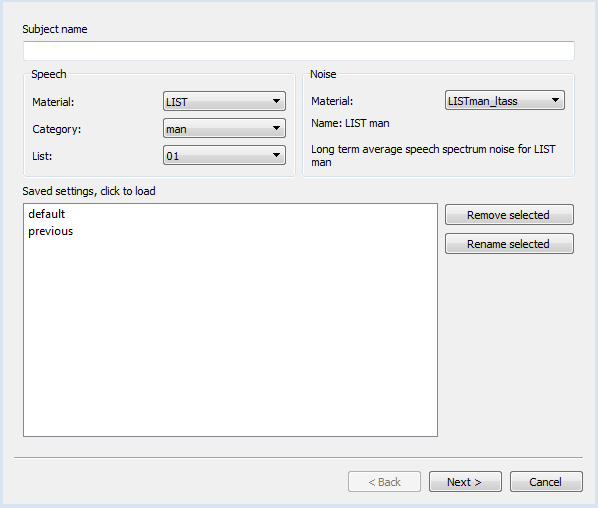
\includegraphics[width=0.5\textwidth]{spin-main}
\caption{Main window of the APEX/SPIN GUI: selection of speech material, noise and saving of settings.}
\label{fig:main} \end{figure} 

On the first page of the GUI, the speech material to be used is
selected (see figure~\ref{fig:main}). All speech materials consist of
lists of tokens, but some materials have additional subdivisions, such
as different speakers. Such subdivisions are called categories, which
can also be selected in the GUI. In figure~\ref{fig:main}, list 1 from
the LIST speech material is selected, using the male speaker (category
``man''). The masker (noise) is in this example the
long-term-average-speech-spectrum noise supplied with the LIST speech
material. Any combination of speech material and noise can be freely
selected. \hl{changed: Custom speech materials or noises can be added (see manual for the procedure)}. Below the speech material
selection elements, one has the possibility to save a set of SPIN
settings for later use. For instance, if one often uses the LIST
material in noise under headphones with an adaptive procedure, these
settings can be saved and loaded later on with a single click.

\begin{figure}
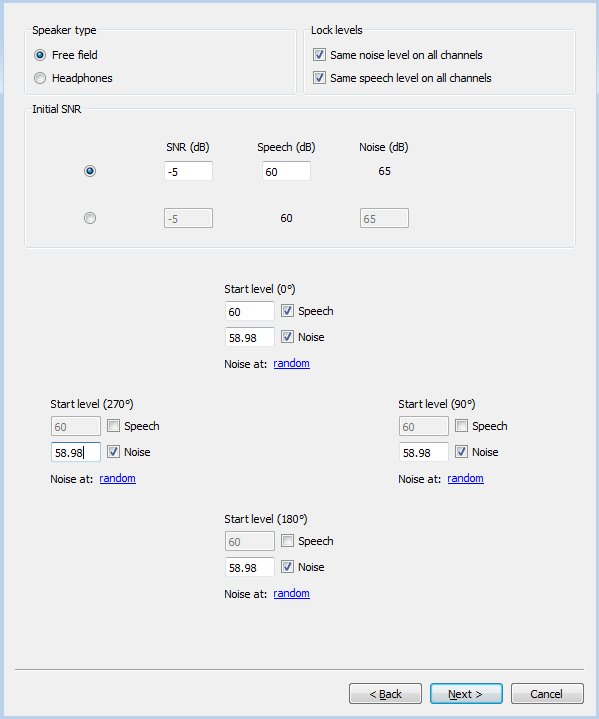
\includegraphics[width=0.45\textwidth]{spin-speakers-ff}
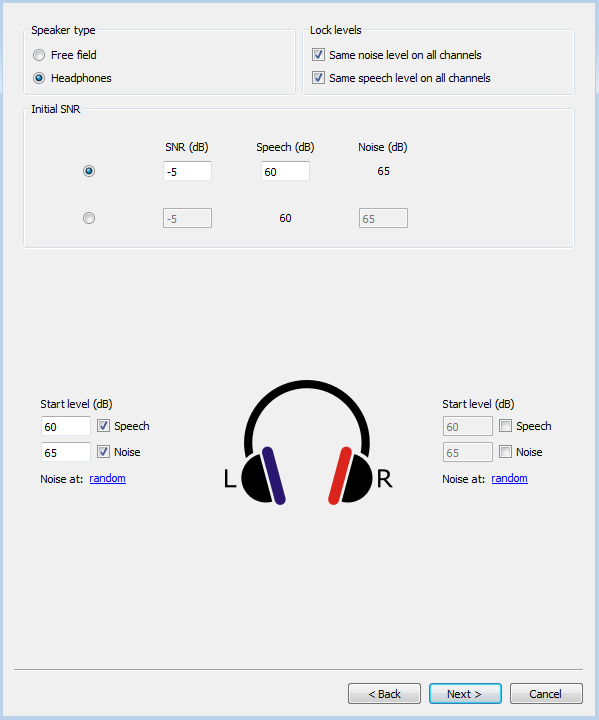
\includegraphics[width=0.45\textwidth]{spin-speakers-headphones}
\caption{Loudspeaker selection: if "speaker type" is set to free field, the left dialog is shown. If "speaker type" is set to headphones, the right dialog is shown. For each loudspeaker or ear, speech and noise can be turned on or off using the check boxes. If the overall SNR or level is specified, the individual levels will be calculated automatically. The "random" link next to each loudspeaker can be used to indicate that the noise should be started at a random place in the provided wav file.}
\label{fig:speaker}
\end{figure}

On the second page (Speakers), the loudspeakers or headphones to be used
can be specified (see figure~\ref{fig:speaker}). First, free
field or headphone stimulation has to be selected. For headphone or
single-loudspeaker free field stimulation, the overall speech and noise
level obviously correspond to the speech and noise level specified for
one ear or for one loudspeaker (right panel of Figure 2). In free field mode, one can either
specify the overall speech and noise level, and then speech and noise
levels for the individual loudspeakers are automatically calculated, by
adding power in linear units (assuming that the noise is uncorrelated
across loudspeakers) and converting back to decibels. An example is shown in the left panel of Figure 2. Alternatively,
speech and noise levels can be specified separately for each ear or
loudspeaker. 

 \begin{figure} 
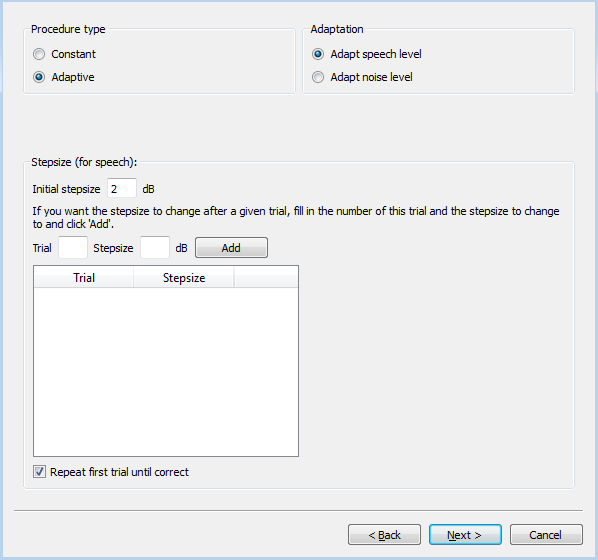
\includegraphics[width=0.5\textwidth]{spin-procedure-adaptive}
\caption{GUI for setting parameters of the adaptive procedure. For the constant procedure, no additional parameters can be specified. }
\label{fig:procedure} \end{figure} 

On the third page, procedural parameters can be entered (see
figure~\ref{fig:procedure}). For constant procedures there are no
parameters, but for adaptive procedures, the step size (in dB) can be
specified, and there is an option to repeat the first token until a
correct answer is given \citep{pm760724} in order not to use too many tokens at SNRs far from
the SRT. On the top right, the user can indicate whether the speech
level should be adapted, in which case the noise level will be fixed
throughout the experiment, or whether the noise level should be adapted,
in which case the speech level will be fixed. A fixed noise level is
often used when testing noise suppression algorithms. A fixed speech
level is often used when the speech needs to fit within a
hearing-impaired subject's limited dynamic range. The starting value of
the parameter that is adapted (speech or noise level) is determined by
the values entered in the Speakers tab.

 \begin{figure} 
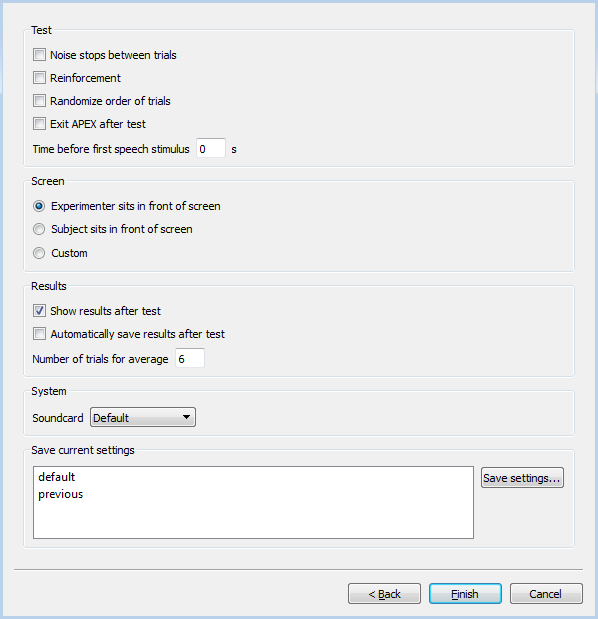
\includegraphics[width=0.5\textwidth]{spin-options}
\caption{GUI for setting various options} \label{fig:options}
\end{figure} 

Finally, on the fourth page, various options can be specified (see
figure~\ref{fig:options}). Most options are self-explanatory.

\begin{description}
\itemsep1pt\parskip0pt\parsep0pt
\item[Noise stops between trials]
If checked, the background noise will be started 1~s before the speech
token starts, and be stopped 1~s after the end of the speech token.
Otherwise, the noise continues throughout the experiment.
\item[Reinforcement]
If checked, the subject will receive visual feedback after each trial:
if the response was correct, a green thumbs-up symbol will be shown, and
if the response was incorrect a red thumbs-down symbol.
\item[Screen]
If there is a test leader present who controls the computer, the correct
response and current SNR will be shown on the screen, together with
buttons to indicate whether the response was correct or false. If the
subject controls the computer, the correct response will not be shown,
but a text box will be shown in which the subject can type the response.
Alternatively, a custom screen can be defined (see
section~\ref{customising}).
\item[Show results after test]
If checked, a graphical display of the results will be shown after the
test, and in case of an adaptive procedure, the SRT will be calculated
as the average of the ``Number of trials for average'' last SNRs
presented.
\end{description}

When all tabs have been completed, the user can press the ``create
experiment'' button. An experiment file will then be generated, and APEX
will query where it should be saved on disk. If the experiment file is stored together 
with the results file, all experimental parameters can be retrieved later on. 



\section{Calibration}
\label{sec:Calibration}

 \begin{figure} 
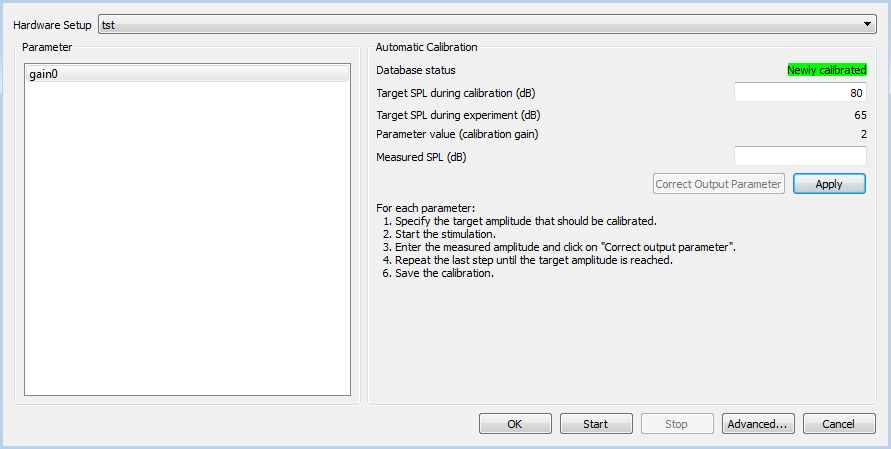
\includegraphics[width=0.5\textwidth]{spin-calibration}
\caption{Calibration dialog. In this example there is only one loudspeaker and its level has been calibrated (indicated by the green message). }
\label{fig:calibration} \end{figure} 

For calibration, the APEX calibration infrastructure is used
\citep{Francart2008}. In summary, during calibration the value of an
APEX parameter (e.g., gain of the first channel of the sound card) is
linked to a sound pressure level, measured with a sound level meter,
entered by the user. Calibration values are stored in a database for
each combination of \emph{hardware setup} and \emph{calibration
profile}. The hardware setup is a string that describes the external
hardware attached to the computer, for example, type of sound card or type of
headphones. It is shown at the top of the calibration dialog (see
figure~\ref{fig:calibration}). With APEX/SPIN, a different calibration
profile is generated for each combination of speech material and noise.
The noise is used as the calibration stimulus. In most cases this will
be the long term average speech spectrum noise accompanying the speech
material. When no calibration value is found in the database for the
current hardware setup and calibration profile, APEX will automatically
present the calibration window. Thereafter, the user can recalibrate at
any time using the calibration menu.

 From the calibration dialog, proceed as follows to calibrate:

\begin{itemize}
\itemsep1pt\parskip0pt\parsep0pt
\item
  Set up the sound level meter to measure the output of the headphones
  (using an artificial ear and pressure gradient microphone), or
  loudspeakers (using a free field microphone) and make sure the sound
  level meter is properly calibrated.
\item
  Select the parameter to be calibrated from the list. Parameters are
  numbered according to output channel. For headphones, 0 is the left
  ear and 1 is the right ear. Loudspeakers are numbered from 0 to the
  number of loudspeakers minus one.
\item
  Press ``start'', the noise will now be looped.
\item
  Read the sound pressure level (in dB~A or dB~SPL) from the sound level
  meter, and enter it in the ``measured amplitude'' box. Note that APEX
  does not store the measurement unit. It is the user's responsibility
  to use consistent units.
\item
  Press ``apply''. The sound level will now be adjusted in order to
  achieve the target level (``calibration amplitude'').
\item
  Check if the measured sound pressure level now corresponds to the
  target level. If it does, press ``apply''. Otherwise, repeat the
  latter two steps above.
\item
 Repeat for each parameter in the list.
\end{itemize}

The ``output parameter'' value will be used by APEX to set the sound to
the desired level. For example, if the calibration amplitude was 80~dB~A, with
corresponding output parameter of 2~dB, and the user requests a speech
level of 60~dB~A, APEX will set the parameter to $60-80+2=-18$~dB during
the experiment.

Note that a noise needs to be defined for each loudspeaker to be
calibrated. If you want to calibrate a speech in quiet experiment, first
create the same experiment with noise on each loudspeaker (check the
relevant check box in the ``Speakers'' tab), start the experiment,
calibrate, exit, and then start the speech in quiet experiment.

Also note that if you recalibrate for an existing hardware setup, you
need to recalibrate for each combination of speech material and noise
that will be used.


\section {Adding speech materials and
noises}
\label{sec:Adding-speech-materials-and-noises}


Our lab provides a number of speech materials in a format readily usable
with APEX/SPIN, including LIST and LINT \citep{VanWieringen2008a},
LIST-m \citep{Jansen2014}, FIST \citep{Luts2008} and FrMatrix
\citep{Jansen2012}, NVA \citep{Wouters1994}, VU \citep{Versfeld2000}
HINT \citep{pm8132902}.

Alternatively, users can easily add their own speech materials and
noises. This involves creating an XML file with the required
information. For each speech material, a separate XML file can be put in
folder \texttt{config} in the APEX path, named
speechmaterial\_\emph{MySpeechMaterial}.xml. An example speech material
file is shown below:

\begin{lstlisting}[caption=Adding a speech material and noise]
<apex:speechmaterialfile>
    <noises>
        <noise id="NoiseId">
            <description>Human readable description of noise</description>
            <name>Noise name</name>
            <uri>mymaterial/ltass.wav</uri>
            <rms>-21.6</rms>
            <speechmaterial>MyMaterial</speechmaterial>
        </noise>
    </noises>
    
    <speechmaterial id="MyMaterial">
        <rms>-25</rms>
        <list id="1">
            <speechtoken id="1">
                <uri>mymaterial/sentence1.wav</uri>
                <text>First Sentence</text>
            </speechtoken>
            ...
        </list>
        ...
    </speechmaterial>
</apex:speechmaterialfile>
\end{lstlisting}

First a noise is defined that will be linked to the speech material.
This is typically long-term-average-speech-spectrum-weighted noise
corresponding to the speech material. Below, the speech material is
defined. Note that the file names next to \texttt{<uri>} are relative to
the speechmaterials prefix (see section~\ref{sec:installation}). The
\texttt{<text>} of each token can be shown on screen during the
experiment to allow scoring. Both the noise and speech material have a
tag \texttt{<rms>}, which defines the root-mean-square (RMS) level in
dB~FS, and will be used to match noise and speech levels. For example, for the
RMS levels in the example, and a desired SNR of 0~dB the noise would be
attenuated relative to the speech by $-25+21.6=3.4$~dB.

To add a noise that is not linked to a speech material, for example, ICRA noise
\citep{Dreschler}, babble noise or competing talker \citep{flucnoise},
it can be added to any speech material file or to the \texttt{spin.xml}
file as illustrated above. In this case, the element
\texttt{<speechmaterial>} needs to be omitted.

\section{Customising}
\label{sec:customising}

APEX/SPIN has some settings that cannot be set in the GUI, but can be
configured by advanced users. This is done by editing the
\texttt{config/spin.xml} file in the APEX path. Some examples are given
below.

\begin{lstlisting}[caption=Specifying speaker locations and a custom screen]
<apex:spin>
    ...
    <speaker_setup>
        <speaker> 
            <angle>0</angle>    
            <channel>0</channel>
        </speaker>
        <speaker>
            <angle>90</angle>
            <channel>1</channel>
        </speaker>
    </speaker_setup>
    ...
    <subject_screen>
        <screen id="subject_screen">
            <gridLayout height="2" width="1" id="main_layout">
                <label x="1" y="1" id="helplabel">
                    <text>Type what you hear</text>
                </label>
                <textEdit x="1" y="2" id="text"/>
            </gridLayout>
            <default_answer_element>text</default_answer_element>
        </screen>
    </subject_screen>
    ...
</apex:spin>
\end{lstlisting}

Under \texttt{<speaker\_setup>}, speaker angles (relative to the
subject, 0 degrees means in front of the subject, 90 degrees to the
right of the subject) are associated with sound card channels, numbered
from 0. This should reflect the physical connections from the sound card
to the loudspeakers. Under \texttt{<subject\_screen>}, the screen layout
during testing is defined, for the case where the subject sits in front
of the screen. Here one could, for instance, translate the text or
customise the look and feel. The remaining options of the spin.xml file
are documented in its associated schema file, \texttt{spin.xsd}.

To customise the way results are analysed and shown, one can edit the
HTML5 file that is used by APEX for this purpose. This file is called
\texttt{config/rtresults.html} under the APEX path.

If further customisations are required that are not available in the GUI
or \texttt{spin.xml} file, there are two remaining options: editing the
experiment file generated by APEX/SPIN, or changing the source code of
APEX/SPIN itself, which is freely available.


\section{Processing results}\label{processing-results}

The option ``Show results after test'' can be selected in the APEX/SPIN dialog. When a results file is opened in APEX at a later stage,
the same analysis is shown. The full results file should be stored
such that additional information that may be required at a
later time for further analysis, such as reaction times, is still available. From this analysis,
one can simply note the required value (e.g., the SRT or percentage
correct), print the results, export to PDF, or copy the raw data to
another program.  Alternatively to copying the results manually, one can
automatically collect the results. For example, data can be exported to the comma separated values (CSV) format
 or can be processed directly with the APEX Matlab Toolbox (e.g., \texttt{a3speechresults.m}) or APEX R Toolbox that come bundled with APEX.
